%╔════════════════════════════╗
%║	  Szablon dostosował	  ║
%║	mgr inż. Dawid Kotlarski  ║
%║		  06.10.2024		  ║
%╚════════════════════════════╝
\documentclass[12pt,twoside,a4paper,openany]{article}

    % ------------------------------------------------------------------------
% PAKIETY
% ------------------------------------------------------------------------

%różne pakiety matematyczne, warto przejrzeć dokumentację, muszą być powyżej ustawień językowych.
\usepackage{mathrsfs}   %Różne symbole matematyczne opisane w katalogu ~\doc\latex\comprehensive. Zamienia \mathcal{L} ze zwykłego L na L-transformatę.
\usepackage{eucal}      %Różne symbole matematyczne.
\usepackage{amssymb}    %Różne symbole matematyczne.
\usepackage{amsmath}    %Dodatkowe funkcje matematyczne, np. polecenie \dfac{}{} skladajace ulamek w trybie wystawionym (porównaj $\dfrac{1}{2}$, a $\frac{1}{2}$).

%język polski i klawiatura
\usepackage[polish]{babel}
%\usepackage{qtimes} % czcionka Times new Roman
\usepackage[OT4]{polski}
%\usepackage[cp1250]{inputenc}                       %Strona kodowa polskich znaków.

%obsługa pdf'a
\usepackage[pdftex,usenames,dvipsnames]{color}      %Obsługa kolorów. Opcje usenames i dvipsnames wprowadzają dodatkowe nazwy kolorow.
\usepackage[pdftex,pagebackref=false,draft=false,pdfpagelabels=false,colorlinks=true,urlcolor=blue,linkcolor=black,citecolor=green,pdfstartview=FitH,pdfstartpage=1,pdfpagemode=UseOutlines,bookmarks=true,bookmarksopen=true,bookmarksopenlevel=2,bookmarksnumbered=true,pdfauthor={Dawid Kotlarski},pdftitle={Dokumentacja Projektowa},pdfsubject={},pdfkeywords={transient recovery voltage trv},unicode=true]{hyperref}   %Opcja pagebackref=true dotyczy bibliografii: pokazuje w spisie literatury numery stron, na których odwołano się do danej pozycji.

%bibliografia
%\usepackage[numbers,sort&compress]{natbib}  %Porządkuje zawartość odnośników do literatury, np. [2-4,6]. Musi być pod pdf'em, a styl bibliogfafii musi mieć nazwę z dodatkiem 'nat', np. \bibliographystyle{unsrtnat} (w kolejności cytowania).
\usepackage[
	backend=biber,
	style=numeric,
	sorting=none
]{biblatex}
\addbibresource{bibliografia.bib}
\usepackage{hypernat}                       %Potrzebna pakietowi natbib do wspolpracy z pakietem hyperref (wazna kolejnosc: 1. hyperref, 2. natbib, 3. hypernat).

%grafika i geometria strony
\usepackage{extsizes}           %Dostepne inne rozmiary czcionek, np. 14 w poleceniu: \documentclass[14pt]{article}.
\usepackage[final]{graphicx}
\usepackage[a4paper,left=3.5cm,right=2.5cm,top=2.5cm,bottom=2.5cm]{geometry}

%strona tytułowa
\usepackage{strona_tytulowa}

%inne
\usepackage[hide]{todo}                     %Wprowadza polecenie \todo{treść}. Opcje pakietu: hide/show. Polecenie \todos ma byc na koncu dokumentu, wszystkie \todo{} po \todos sa ignorowane.
\usepackage[basic,physics]{circ}            %Wprowadza środowisko circuit do rysowania obwodów elektrycznych. Musi byc poniżej pakietow językowych.
\usepackage[sf,bf,outermarks]{titlesec}     %Troszczy się o wygląd tytułów rozdziałów (section, subsection, ...). sf oznacza czcionkę sans serif (typu arial), bf -- bold. U mnie: oddzielna linia dla naglowku paragraph. Patrz tez: tocloft -- lepiej robi format spisu tresci.
\usepackage{tocloft}                        %Troszczy się o format spisu trsci.
\usepackage{expdlist}    %Zmienia definicję środowiska description, daje większe możliwości wpływu na wygląd listy.
\usepackage{flafter}     %Wprowadza parametr [tb] do polecenia \suppressfloats[t] (polecenie to powoduje nie umieszczanie rysunkow, tabel itp. na stronach, na ktorych jest to polecenie (np. moze byc to stroma z tytulem rozdzialu, ktory chcemy zeby byl u samej gory, a nie np. pod rysunkiem)).
\usepackage{array}       %Ładniej drukuje tabelki (np. daje wiecej miejsca w komorkach -- nie są tak ścieśnione, jak bez tego pakietu).
\usepackage{listings}    %Listingi programow.
\usepackage[format=hang,labelsep=period,labelfont={bf,small},textfont=small]{caption}   %Formatuje podpisy pod rysunkami i tabelami. Parametr 'hang' powoduje wcięcie kolejnych linii podpisu na szerokosc nazwy podpisu, np. 'Rysunek 1.'.
\usepackage{appendix}    %Troszczy się o załączniki.
\usepackage{floatflt}    %Troszczy się o oblewanie rysunkow tekstem.
\usepackage{here}        %Wprowadza dodtkowy parametr umiejscowienia rysunków, tabel, itp.: H (duże). Umiejscawia obiekty ruchome dokladnie tam gdzie są w kodzie źródłowym dokumentu.
\usepackage{makeidx}     %Troszczy się o indeks (skorowidz).

%nieużywane, ale potencjalnie przydatne
\usepackage{sectsty}           %Formatuje nagłówki, np. żeby były kolorowe -- polecenie: \allsectionsfont{\color{Blue}}.
%\usepackage{version}           %Wersje dokumentu.

%============
\usepackage{longtable}			%tabelka
%============

%============
% Ustawienia listingów do kodu
%============

\usepackage{listings}
\usepackage{xcolor}

\definecolor{codegreen}{rgb}{0,0.6,0}
\definecolor{codegray}{rgb}{0.5,0.5,0.5}
\definecolor{codepurple}{rgb}{0.58,0,0.82}
\definecolor{backcolour}{rgb}{0.95,0.95,0.92}

% Definicja stylu "mystyle"
\lstdefinestyle{mystyle}{
	backgroundcolor=\color{backcolour},
	commentstyle=\color{codegreen},
	keywordstyle=\color{blue},	%magenta
	numberstyle=\tiny\color{codegray},
	stringstyle=\color{codepurple},
	basicstyle=\ttfamily\footnotesize,
	breakatwhitespace=false,
	breaklines=true,
	captionpos=b,
	keepspaces=true,
	numbers=left,
	numbersep=5pt,
	showspaces=false,
	showstringspaces=false,
	showtabs=false,
	tabsize=2
}

\lstset{style=mystyle} % Deklaracja aktywnego stylu
%===========

%PAGINA GÓRNA I DOLNA
\usepackage{fancyhdr}          %Dodaje naglowki jakie się chce.
\pagestyle{fancy}
\fancyhf{}
% numery stron w paginie dolnej na srodku
\fancyfoot[C]{\scriptsize DOKUMENTACJA PROJEKTU - ZAAWANSOWANE PROGRAMOWANIE \\
	\normalsize\sffamily  \thepage}


%\fancyhead[L]{\small\sffamily \nouppercase{\leftmark}}
\fancyhead[C]{\footnotesize \textit{AKADEMIA NAUK STOSOWANYCH W NOWYM SĄCZU}\\}

\renewcommand{\headrulewidth}{0.4pt}
\renewcommand{\footrulewidth}{0.4pt}

    % ------------------------------------------------------------------------
% USTAWIENIA
% ------------------------------------------------------------------------

% ------------------------------------------------------------------------
%   Kropki po numerach sekcji, podsekcji, itd.
%   Np. 1.2. Tytuł podrozdziału
% ------------------------------------------------------------------------
\makeatletter
    \def\numberline#1{\hb@xt@\@tempdima{#1.\hfil}}                      %kropki w spisie treści
    \renewcommand*\@seccntformat[1]{\csname the#1\endcsname.\enspace}   %kropki w treści dokumentu
\makeatother

% ------------------------------------------------------------------------
%   Numeracja równań, rysunków i tabel
%   Np.: (1.2), gdzie:
%   1 - numer sekcji, 2 - numer równania, rysunku, tabeli
%   Uwaga ogólna: o otoczeniu figure ma być najpierw \caption{}, potem \label{}, inaczej odnośnik nie działa!
% ------------------------------------------------------------------------
\makeatletter
    \@addtoreset{equation}{section} %resetuje licznik po rozpoczęciu nowej sekcji
    \renewcommand{\theequation}{{\thesection}.\@arabic\c@equation} %dodaje kropki

    \@addtoreset{figure}{section}
    \renewcommand{\thefigure}{{\thesection}.\@arabic\c@figure}

    \@addtoreset{table}{section}
    \renewcommand{\thetable}{{\thesection}.\@arabic\c@table}
\makeatother

% ------------------------------------------------------------------------
% Tablica
% ------------------------------------------------------------------------
\newenvironment{tabela}[3]
{
    \begin{table}[!htb]
    \centering
    \caption[#1]{#2}
    \vskip 9pt
    #3
}{
    \end{table}
}

% ------------------------------------------------------------------------
% Dostosowanie wyglądu pozycji listy \todos, np. zamiast 'p.' jest 'str.'
% ------------------------------------------------------------------------
\renewcommand{\todoitem}[2]{%
    \item \label{todo:\thetodo}%
    \ifx#1\todomark%
        \else\textbf{#1 }%
    \fi%
    (str.~\pageref{todopage:\thetodo})\ #2}
\renewcommand{\todoname}{Do zrobienia...}
\renewcommand{\todomark}{~uzupełnić}

% ------------------------------------------------------------------------
% Definicje
% ------------------------------------------------------------------------
\def\nonumsection#1{%
    \section*{#1}%
    \addcontentsline{toc}{section}{#1}%
    }
\def\nonumsubsection#1{%
    \subsection*{#1}%
    \addcontentsline{toc}{subsection}{#1}%
    }
\reversemarginpar %umieszcza notki po lewej stronie, czyli tam gdzie jest więcej miejsca
\def\notka#1{%
    \marginpar{\footnotesize{#1}}%
    }
\def\mathcal#1{%
    \mathscr{#1}%
    }
\newcommand{\atp}{ATP/EMTP} % Inaczej: \def\atp{ATP/EMTP}

% ------------------------------------------------------------------------
% Inne
% ------------------------------------------------------------------------
\frenchspacing                      
\hyphenation{ATP/-EMTP}             %dzielenie wyrazu w danym miejscu
\setlength{\parskip}{3pt}           %odstęp pomiędzy akapitami
\linespread{1.3}                    %odstęp pomiędzy liniami (interlinia)
\setcounter{tocdepth}{4}            %uwzględnianie w spisie treści czterech poziomów sekcji
\setcounter{secnumdepth}{4}         %numerowanie do czwartego poziomu sekcji 
\titleformat{\paragraph}[hang]      %wygląd nagłówków
{\normalfont\sffamily\bfseries}{\theparagraph}{1em}{}

% Makro do zdjęć
\newcommand*{\fg}[4][!htb]{
    \begin{figure}[#1]
        \begin{center}
            \includegraphics[width=8cm]{#2}
            \caption{#3}
            \label{#4}
        \end{center}
    \end{figure}
}


    %polecenia zdefiniowane w pakiecie strona_tytulowa.sty
    \title{...Algorytm listy dwukierunkowej \\z zastosowaniem GitHub...}		%...Wpisać nazwę projektu...
    \author{Mateusz Basiaga}
    \authorI{}
    \authorII{}		%jeśli są dwie osoby w projekcie to zostawiamy:    \authorII{}
		
	\uczelnia{AKADEMIA NAUK STOSOWANYCH \\W NOWYM SĄCZU}
    \instytut{Wydział Nauk Inżynieryjnych}
    \kierunek{Katedra Informatyki}
    \praca{DOKUMENTACJA PROJEKTOWA}
    \przedmiot{ZAAWANSOWANE PROGRAMOWANIE}
    \prowadzacy{mgr inż. Dawid Kotlarski}
    \rok{2024}


%definicja składni mikrotik
\usepackage{fancyvrb}
\DefineVerbatimEnvironment{MT}{Verbatim}%
{commandchars=\+\[\],fontsize=\small,formatcom=\color{red},frame=lines,baselinestretch=1,} 
\let\mt\verb 
%zakonczenie definicji składni mikrotik

\usepackage{fancyhdr}    %biblioteka do nagłówka i stopki

			
\begin{document}
   
    \renewcommand{\figurename}{Rys.}    %musi byc pod \begin{document}, bo w~tym miejscu pakiet 'babel' narzuca swoje ustawienia
    \renewcommand{\tablename}{Tab.}     %j.w.
    \thispagestyle{empty}               %na tej stronie: brak numeru
    \stronatytulowa                     %strona tytułowa tworzona przez pakiet strona_tytulowa.tex
 
 \pagestyle{fancy}

    \newpage

    %formatowanie spisu treści i~nagłówków
    \renewcommand{\cftbeforesecskip}{8pt}
    \renewcommand{\cftsecafterpnum}{\vskip 8pt}
    \renewcommand{\cftparskip}{3pt}
    \renewcommand{\cfttoctitlefont}{\Large\bfseries\sffamily}
    \renewcommand{\cftsecfont}{\bfseries\sffamily}
    \renewcommand{\cftsubsecfont}{\sffamily}
    \renewcommand{\cftsubsubsecfont}{\sffamily}
    \renewcommand{\cftparafont}{\sffamily}
    %koniec formatowania spisu treści i nagłówków
     
    \tableofcontents    %spis treści
    \thispagestyle{fancy}
    \newpage

    
    \newpage

    
%%%%%%%%%%%%%%%%%%% treść główna dokumentu %%%%%%%%%%%%%%%%%%%%%%%%%

   	\newpage
\section{Ogólne określenie wymagań}		%1
%Określenie celu pracy, co chcemy uzyskać, jakie przewidujemy wyniki













\hspace{0.60cm}Tutaj może coś być wpisane. 

\subsection{Przykład}  %1.1       

\hspace{0.60cm}Tak zaczynamy pisanie pierwszego akapitu. Jeśli chcemy napisać przypis do bibliografii wykonujemy to w~ten sposób\footnote{Przykład odnośnika do książki\cite{legierski}.}.

%rysunek
	\begin{figure}[!htb]
	\begin{center}
		
\includegraphics[width=8cm]{rys/ans.png}
		\caption{Logo}
		\label{rys:rysunek001}
	\end{center}
\end{figure}

Tutaj może coś być wpisane. \\Tutaj może coś być wpisane\footnote{Przykład odnośnika do strony www\cite{www1}.}. 
Rysunek \ref{rys:rysunek001} (s. \pageref{rys:rysunek001}) pokazuje przykładową ilustrację.

%tabelka
\begin{tabela}
	%uwaga: w nawiasach [] nie może być odnośnika do literatury, jeżeli w dokumencie jest spis rysunków na początku, a spis literatury jest w kolejności cytowania (zmienia to numeracji)
	{Tabelka przykładowa}	%opis w spisie tabel
	{Tabelka przykładowa}	%opis przy tabeli
	{
		\begin{tabular}{|c|c|} \hline
			$U_n$ & $I_{zw}$ \\ \hline
			$kV$  & $\%$      \\ \hline
			7.2 & 100 \\ \hline
		\end{tabular}
	}
	\label{tab:tablica001}
\end{tabela}

% Kod

Listing kodu

\begin{lstlisting}[caption=Przykładowy kod 001, label={lst:listing-cpp}, language=C++]
#include <iostream>
#include <cstdlib>
#include <ctime>
using namespace std;

/*
liczby pseldolosowe
*/

int main(int argc, char** argv) {
	
	int tab[10][10];
	
	for(int i=0;i<10;i++)
	for(int j=0;j<10;j++)
	tab[i][j]=0;
	
	srand(time(NULL));		//generowanie z czasu
	int min=3;
	int max=7;
	for(int i=0;i<10;i++)
	for(int j=0;j<10;j++)		
	tab[i][j]=(rand()%(max-min+1))+min;	
	
	for(int i=0;i<10;i++)
	{
		for(int j=0;j<10;j++)
		cout<<tab[i][j]<<" ";	
		cout<<endl;
	}
	
	return 0;
}
\end{lstlisting}

Tutaj może coś być wpisane. Tutaj może coś być wpisane. Tutaj może coś być wpisane. Tabela \ref{tab:tablica001} (s. \pageref{tab:tablica001}) pokazuje sposoby użycia trybu matematycznego.

Kod \ref{lst:listing-cpp} (s. \pageref{lst:listing-cpp}) przedstawia sposób generowania liczb pseudolosowych. Kod \ref{lst:listing-cpp2} (s. \pageref{lst:listing-cpp2}) przedstawia generowanie pliku HTML.

Alternatywna metoda wklejenia kodu:

\lstinputlisting[caption=Przykładowy kod 002, label={lst:listing-cpp2}, language=C++]{kod/main.cpp}


\subsection{Instalacja}  %1.2

\hspace{0.60cm}Poniżej są opisane kroki potrzebne do instalacji \LaTeX 'a oraz do używania tego szablonu.

 Na początku instalujemy \TeX{}Live\footnote{Instalka na stronie  https://www.tug.org/texlive/acquire-netinstall.html\cite{www2}.}. Ściągamy plik instalacyjny, zajmuje około 25MB. Podczas instalacji można wybrać do zainstalowania różne kolekcje pakietów. Jeśli nie ma problemów z miejscem na dysku to można zainstalować wszystkie, wtedy nie będzie problemu z brakującymi pakietami i błędami. Po wybraniu kolekcji brakujące pliki są pobierane z internetu. Pełna instalacja programu zajmuje około 8GB. Najlepiej zostawić instalację na noc, ponieważ proces zabiera sporo czasu. Warto ustawić komputer tak, aby się nie wyłączył lub nie uśpił. Warto także przed instalacją zablokować antywirusa, ponieważ może blokować niektóre z komponentów.
 
Następnie instalujemy \TeX{}studio\footnote{Plik instalacyjny na stronie  https://www.texstudio.org\cite{www3}.}. Ściągamy plik instalacyjny zajmujący około 120MB. Instalacja przebiega standardowo.

 %rysunek
\begin{figure}[!hbt]
	\begin{center}
		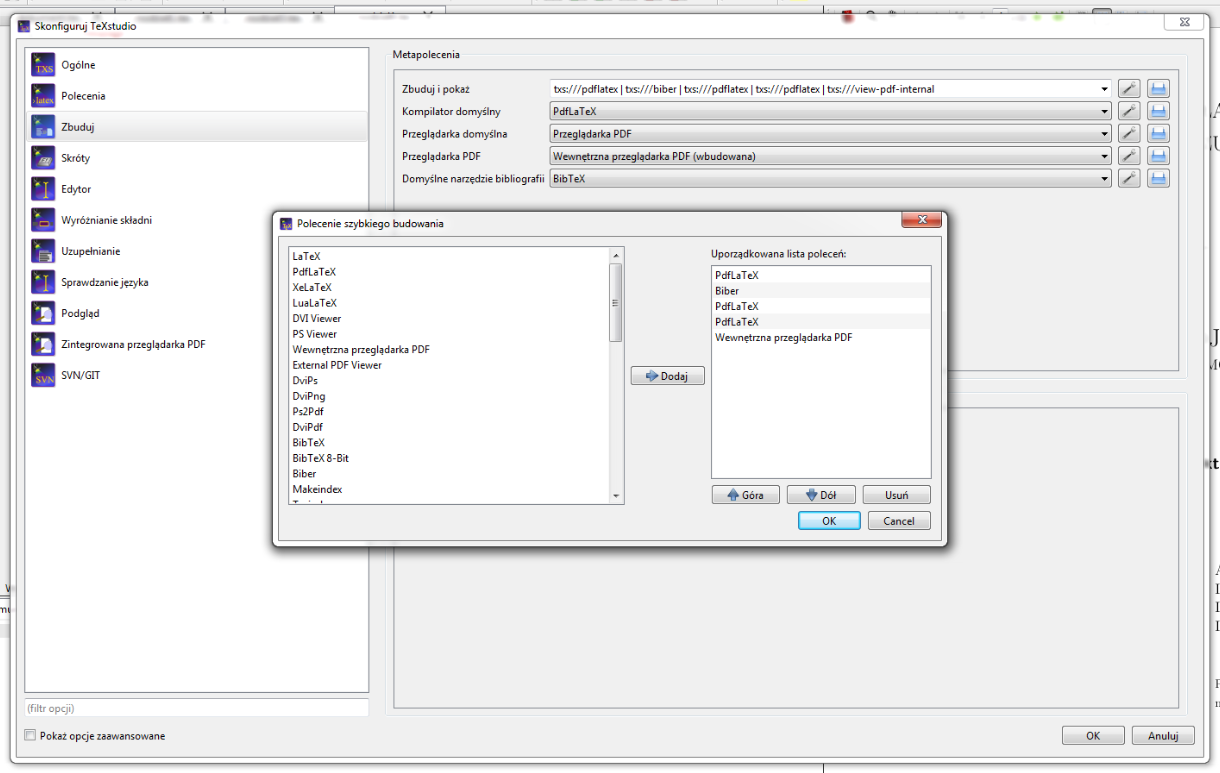
\includegraphics[width=\linewidth]{rys/ustawienie.png}
		\caption{Ustawienie TeXstudio}
		\label{rys:ustawienia}
	\end{center}
\end{figure}

Następnym krokiem jest ustawienie w \TeX{}Studio kolejności budowania projektu. Należy wybrać zakładkę: ,,Opcje/Konfiguruj \TeX{}studio...''. W otwartym oknie przechodzimy na zakładkę ,,Zbuduj''. Na rysunku \ref{rys:ustawienia} (s. \pageref{rys:ustawienia}) pokazany jest zrzut ekranu z konfiguracją. W linijce ,,Zbuduj i pokaż'' klikamy ikonę klucza, żeby przejść do konfiguracji polecenia. W otwartym oknie ustawić kolejność tak jak pokazano na rysunku.

 
 
 
 
 
   \newpage
\section{Analiza problemu}		%2
\hspace{0.60cm}
Lista dwukierunkowa to lista, w której możemy poruszać się w dwóch kierunkach.
Każdy element zawiera co najmniej trzy pola: klucz, prev oraz next. W rezultacie
elementy wskazują zarówno swoje poprzedniki, jak i następniki. Strukturę logiczną listy przedstawiono na rysunku
\textbf{2.1}\footnote{Źródło: Contentplus.pl Sp. z o.o., licencja: CC BY-SA 3.0.}

\begin{figure}[!htb]
  \begin{center}
    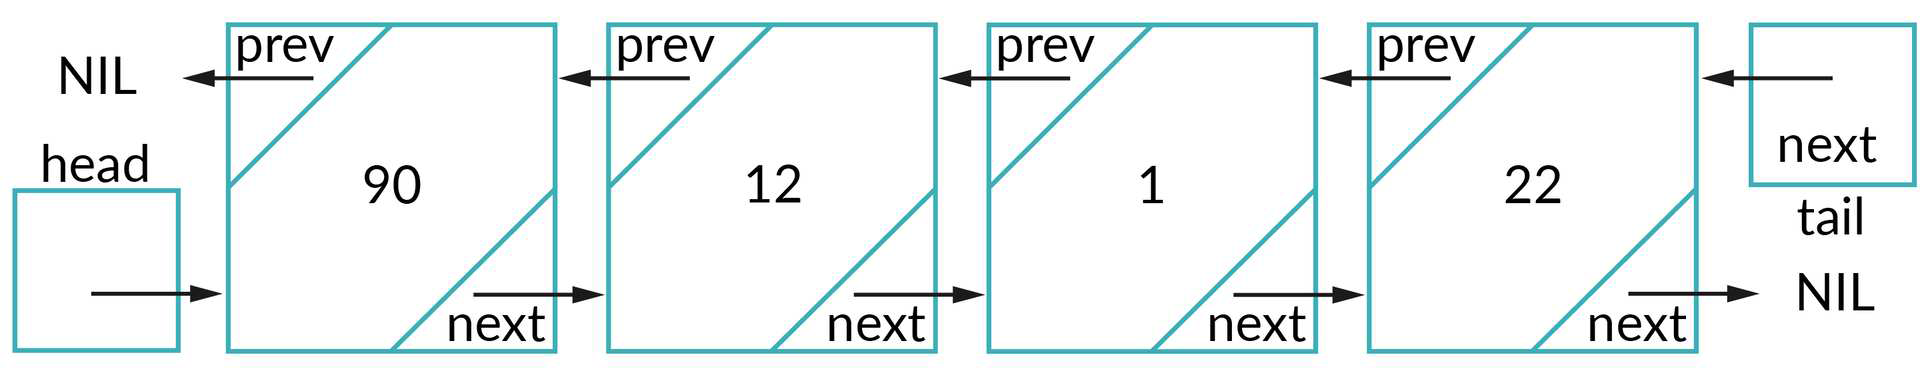
\includegraphics[width=\textwidth]{rys/lista-dwukierunkowa.png}
    \caption{Lista dwukierunkowa}\label{rys:lista_dwukierunkowa}
  \end{center}
\end{figure}

\subsection{Zastosowanie algorytmu listy dwukierunkowej\cite{ZPE}}

Listy dwukierunkowe są szeroko stosowane w różnych dziedzinach informatyki, gdy konieczne jest przechowywanie i manipulowanie dynamicznie zmieniającą się liczbą elementów, przy jednoczesnym zachowaniu możliwości poruszania się w obu kierunkach — do przodu i do tyłu. Typowe zastosowania list dwukierunkowych obejmują:

\begin{itemize}
  \item Implementację struktur takich jak deki (kolejki dwustronne), które pozwalają na dodawanie i usuwanie elementów z obu końców.
  \item Systemy zarządzania pamięcią, gdzie listy dwukierunkowe są używane do śledzenia dostępnych i zajętych bloków pamięci.
  \item Nawigację w przeglądarkach internetowych (przycisk „wstecz” i „dalej”), gdzie konieczne jest poruszanie się w obu kierunkach między odwiedzonymi stronami.
  \item Implementację buforów cyklicznych, gdzie struktura umożliwia płynne przechodzenie pomiędzy początkowym a końcowym elementem listy.
  \item Różne algorytmy wyszukiwania i sortowania, które wymagają przemieszczania się po danych w obu kierunkach.
\end{itemize}

\newpage
\subsection{Działanie listy dwukierunkowej}
\begin{itemize}
  \item \textbf{Wstawianie elementów} na początku, na końcu lub na podanym indeksie.

        Na rysunku \textbf{2.2}\footnote{Zdjęcie ze strony \url{https://www.programiz.com/dsa/doubly-linked-list}\cite{Programiz} \\ (Dostęp: 24.10.2024r.)} pokazano dodawanie elementu na początek listy.

        \begin{figure}[!htb]
          \begin{center}
            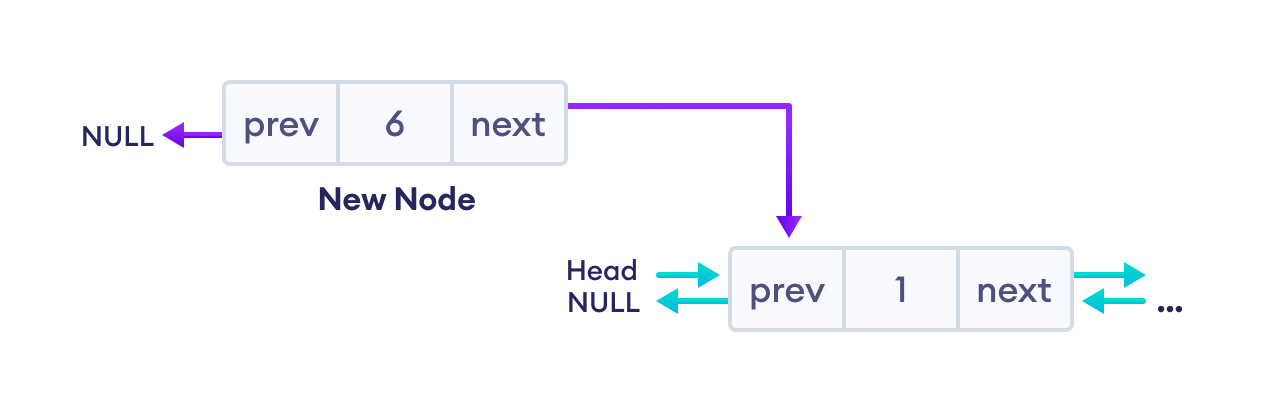
\includegraphics[width=\textwidth]{rys/dodawanie-elementu.png}
            \caption{Dodawanie elementu na początek listy}\label{rys:dodawanie_elementu}
          \end{center}
        \end{figure}

  \item \textbf{Usuwanie elementów} z początku, z końca lub z dowolnej pozycji w liście oraz czyszczenie listy.

        Na rysunku \textbf{2.3}\footnote{Zdjęcie ze strony \url{https://www.programiz.com/dsa/doubly-linked-list}\cite{Programiz} \\ (Dostęp: 24.10.2024r.)} pokazano usuwanie elementu z początku listy.

        \begin{figure}[!htb]
          \begin{center}
            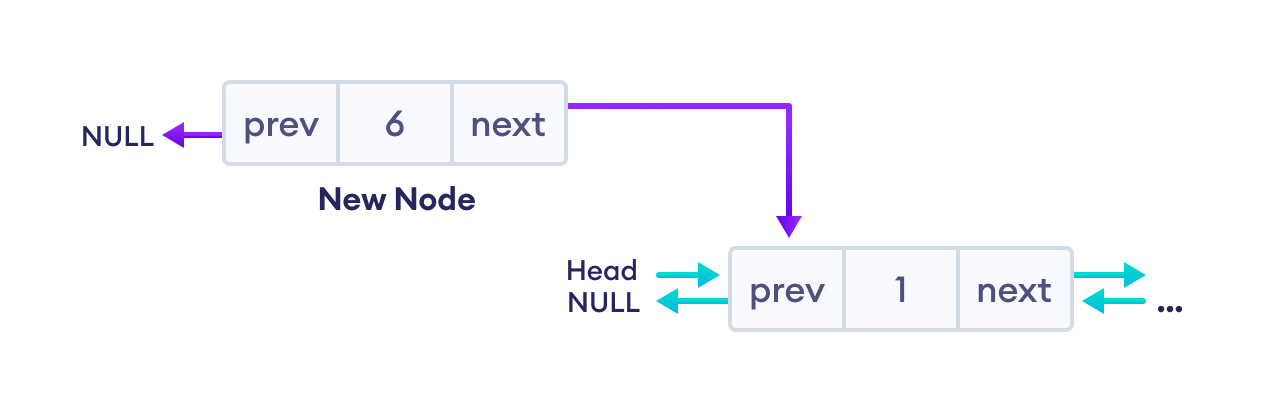
\includegraphics[width=\textwidth]{rys/dodawanie-elementu.png}
            \caption{Usuwanie elementu z początku listy}\label{rys:usuwanie_elementu}
          \end{center}
        \end{figure}

  \item \textbf{Wyświetlanie elementów} zarówno w kolejności od początku do końca, jak i w odwrotnej kolejności.

  \item \textbf{Przeglądanie listy}, zaczynając od określonego indeksu, w obu kierunkach (do przodu lub do tyłu).
\end{itemize}

\newpage

\subsection{Wykorzystanie systemu kontroli wersji Git i platformy GitHub}

\subsubsection[Systemy kontroli wersji]{Systemy kontroli wersji~\cite{ProGit}}

Czym są systemy kontroli wersji?
System kontroli wersji — oprogramowanie służące do śledzenia zmian głównie w kodzie źródłowym oraz pomocy programistom \\ w łączeniu zmian dokonanych w plikach przez wiele osób w różnym czasie.

Dlaczego warto znać systemy kontroli wersji
Proces tworzenia i rozwoju oprogramowania polega na nieustannym wprowadzaniu zmian w kodzie. Nawet jeśli pracujemy w pojedynkę z czasem zarządzanie takimi zmianami przy pomocy naiwnych metod (np. tworzenie nowego katalogu opisanego data i nazwą danej \\ wersji) staje się problematyczne, czasochłonne i na ogół nieefektywne. Nie mamy również łatwej możliwości archiwizacji czy cofania zmian. \\ Problem jest dodatkowo potęgowany kiedy mamy do czynienia z zespołem programistów pracującym nad projektem. Oprócz oczywistej konieczności ciągłego ręcznego przekazywania sobie zmian pojawia się kwestia rozwiązywania nieuniknionych konfliktów. \\ Wtedy właśnie z pomocą przychodzą systemy kontroli wersji.


\subsubsection[Czym jest Git]{Czym jest Git~\cite{ProGit}}
Git — system kontroli wersji utworzony w 2005 roku przez społeczność rozwijającą jądro systemu Linux (a w szczególności Linusa Torvaldsa, twórcę Linuksa)
po tym jak pogorszyły się jej relacje z firmą odpowiedzialną za stworzenie systemu kontroli BitKeeper, którego wówczas używali.
\\
Charakteryzują go przede wszystkim:
\begin{itemize}
  \item Szybkość
  \item Prosta konstrukcja
  \item Silne wsparcie dla nieliniowego rozwoju (tysięcy równoległych gałęzi)
  \item Pełne rozproszenie
  \item Wydajna obsługa dużych projektów, takich jak jądro systemu Linux (szybkość i rozmiar danych)
\end{itemize}

\subsubsection{Platformy hostowania kodu źródłowego}
Najpopularniejsze platformy do hostowania kodu to
\begin{itemize}
  \item \href{https://github.com/}{GitHub}
  \item \href{https://about.gitlab.com/}{GitLab}
  \item \href{https://bitbucket.org/product}{BitBucket}
  \item \href{https://sourceforge.net/}{SourceForge}
\end{itemize}

W tym przypadku skupimy się na platformie GitHub. Warto wspomnieć, że GitHub oferuje studentom darmową subskrypcję Pro do celów edukacyjnych jak również inne pakiety. Więcej na ten temat \href{https://education.github.com/students}{pod adresem}.

   \newpage
\section{Projektowanie}		%3
%Narysować graf, UML, diagram klas, schemat działania algorytmu

\subsection{Narzędzia i technologie}

W projekcie wykorzystano następujące narzędzia i technologie:

\begin{itemize}
  \item \textbf{Język programowania:} C++.
  \item \textbf{Kompilator:} GCC (GNU Compiler Collection) dla systemów Linux oraz MINGW-w64 dla systemu Windows.
  \item \textbf{System budowania:} CMake z użyciem Ninja jako generatora systemu budowania.
  \item \textbf{Dokumentacja:} Narzędzie \texttt{Doxygen} do generowania dokumentacji technicznej oraz szablon \LaTeX{} dostosowany przez mgr inż. Dawida Kotlarskiego.
  \item \textbf{Kontrola wersji:} Git oraz platforma GitHub.
  \item \textbf{Git Hooks:} Lefthook do automatyzacji zadań związanych z Git.
  \item \textbf{Continuous Integration:} GitHub Actions do automatyzacji testów i budowy projektu.
  \item \textbf{Walidacja commitów:} Narzędzie \texttt{Commitlint} do sprawdzania wiadomości commitów zgodnie z konwencją Conventional Commits.
\end{itemize}

\subsection{Ustawienia kompilatora}

Projekt korzysta z systemu CMake, który umożliwia konfigurację i zarządzanie ustawieniami kompilatora dla różnych platform. Ustawienia są dostosowane do pracy z:

\begin{itemize}
  \item \textbf{Windows:} MINGW-w64 z MSYS2 jako środowiskiem terminalowym.
  \item \textbf{Linux:} GCC, który jest standardowym kompilatorem na większości dystrybucji systemu Linux.
\end{itemize}

Dzięki zastosowaniu CMake projekt jest w stanie automatycznie generować odpowiednie pliki Makefile dla Ninja, co umożliwia szybkie i efektywne budowanie aplikacji.

\subsection{Schemat działania programu}

Poniżej przedstawiono diagram UML klas, który ilustruje strukturę i relacje pomiędzy klasami w projekcie.

\begin{figure}[!htb]
  \begin{center}
    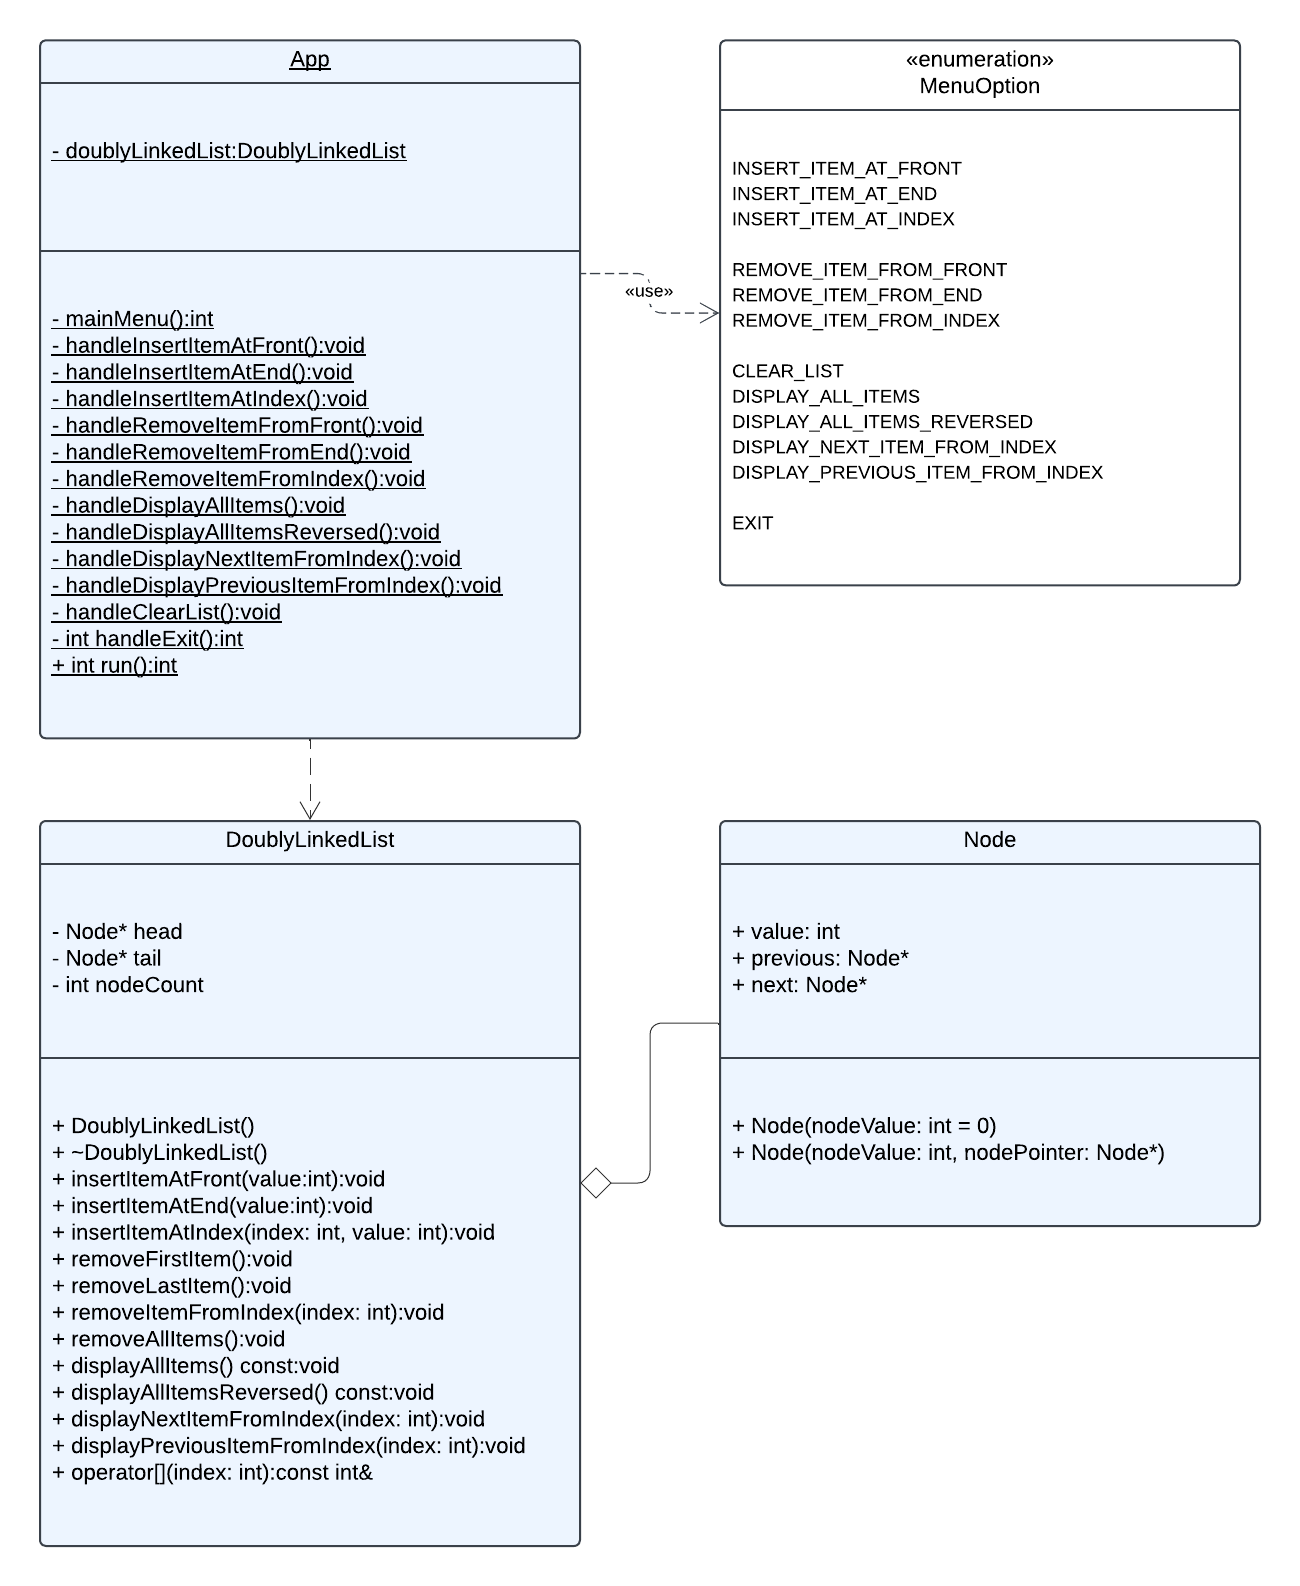
\includegraphics[width=\textwidth]{rys/diagram_UML.png}
    \caption{Diagram UML klas dla projektu}\label{fig:uml_diagram}
  \end{center}
\end{figure}

\subsection{Użycie narzędzi}

Na potrzeby tego i przyszłych projektów o podobnym charakterze
został utworzony szablon repozytorium na platformie GitHub.
Znajduje jest ono pod adresem: \url{https://github.com/Me-Phew/programowanie-zaawansowane-template}\cite{GitHubProjectTemplate} (Dostęp: 24.10.2024r.).
Zawiera następujące funkcjonalności:

\begin{itemize}
  \item \textbf{Generator systemu budowania:} CMake do zarządzania konfiguracją projektu.
  \item \textbf{Kompleksowa konfiguracja dla GCC (MINGW-w64) oraz Linux.}
  \item \textbf{Automatyzacja budowy projektu:} Ninja jako system budowania.
  \item \textbf{Dokumentacja:} Generowana automatycznie z użyciem Doxygen oraz szablonu LaTeX.
  \item \textbf{Zarządzanie tematami:} Temat Doxygen Awesome z kolorami inspirowanymi stroną Nuxt.
  \item \textbf{Git Hooks:} Lefthook do automatyzacji i walidacji wiadomości commitów.
  \item \textbf{Continous Integration:} GitHub Actions do automatyzacji procesów budowy i testowania.
  \item \textbf{Generowanie strony dokumentacji automatycznej:} GitHub Pages.
  \item \textbf{Tworzenie wydań:} Zawierające pliki wykonywalne dla systemów Windows i Linux oraz pliki dokumentacji.
\end{itemize}

\newpage

\subsection{Przykładowa konfiguracja CMake}

Przykładowa konfiguracja pliku \texttt{Zawartość pliku CMakeLists.txt} dla projektu została przedstawiona
na listingu \textbf{3.1}

\begin{lstlisting}[caption=CMakeLists.txt, label={lst:listing-CMakeLists.txt}, language=C++]
cmake_minimum_required(VERSION 3.10)

project(DoublyLinkedList)

include_directories(src/app src/doubly_linked_list)

set(SOURCES src/app/app.cpp src/doubly_linked_list/doubly_linked_list.cpp src/main.cpp)

add_executable(DoublyLinkedList ${SOURCES})

# Compile with all warnings, treat warnings as errors
if (MSVC)
		add_compile_options(/W4 /WX)
else()
		add_compile_options(-Wall -Wextra -pedantic -Werror)
endif()
\end{lstlisting}

Powyższa konfiguracja definiuje minimalną wersję CMake, ustawia standard C++ oraz określa pliki źródłowe projektu.

   \newpage
\section{Implementacja}		%4

\subsection{Struktura Node}

Pierwszym istotnym elementem jest struktura \texttt{Node}, która reprezentuje pojedynczy węzeł \\
w podwójnie powiązanej liście. Definicję klasy \texttt{Node} przedstawiono na listingu \textbf{4.1}:

\lstinputlisting[caption=Struktura Node, label={lst:listing-node.cpp}, language=C++]{kod/node.cpp}

Struktura ta definiuje trzy podstawowe atrybuty: wartość przechowywaną w węźle, wskaźnik na następny węzeł oraz wskaźnik na poprzedni węzeł. Konstruktor inicjalizuje te atrybuty.

\subsection{Klasa DoublyLinkedList}

Główna klasa, \texttt{DoublyLinkedList}, zawiera metody do dodawania, usuwania oraz przeszukiwania węzłów.
Jej strukturę przedstawiono na listingu \textbf{4.2}

\lstinputlisting[caption=Klasa DoublyLinkedList, label={lst:listing-doubly_linked_list.cpp}, language=C++]{kod/doubly_linked_list.cpp}

\subsection{Klasa App}

Klasa App, posiadająca jedynie składowe statyczne odpowiada za uruchomnienie programu i wyświetlanie interfejsu użytkownika.
Jej strukturę przedstawiono na listingu \textbf{4.3}

\lstinputlisting[caption=Klasa App, label={lst:listing-app.cpp}, language=C++]{kod/app.cpp}

\subsection{Wyniki implementacji}

\subsubsection{Obsługa programu}
Na rysunku \textbf{4.1} przedstawiono menu główne programu.

\begin{figure}[!htb]
	\begin{center}
		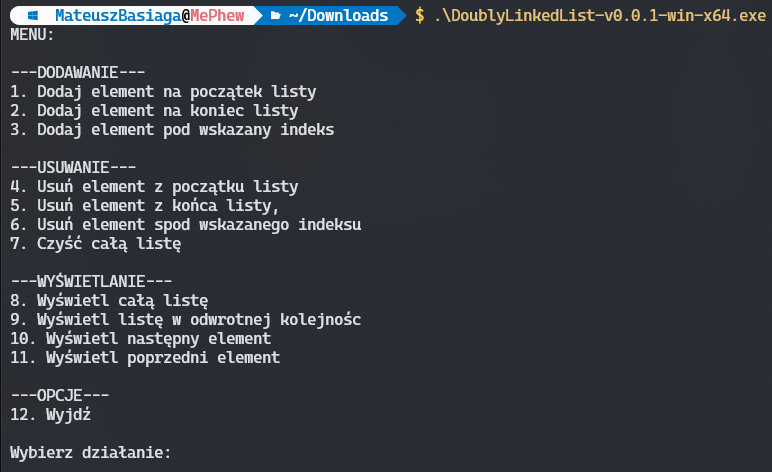
\includegraphics[width=\textwidth]{rys/menu.png}
		\caption{Menu główne programu}\label{rys:menu_programu}
	\end{center}
\end{figure}

\subsection{Wykorzystanie systemu Git i platformy GitHub}

Wdrożono automatyczną publikację nowych wersji programu w ramach systemu CI.
Na rysunku \textbf{4.2} pokazano pierwszą opublikowaną wersję programu.

\begin{figure}[!htb]
	\begin{center}
		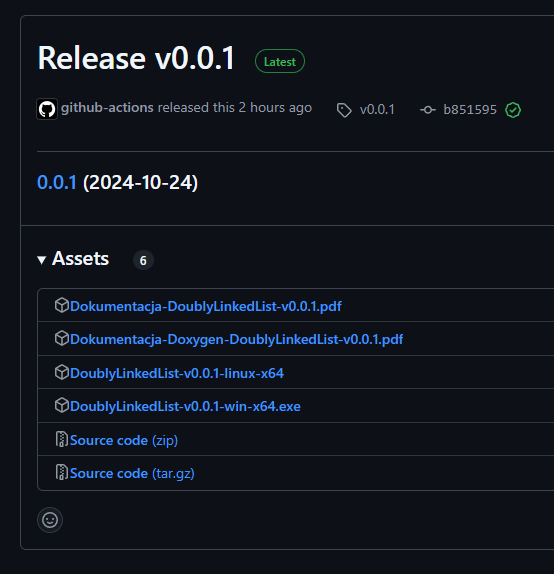
\includegraphics[width=\textwidth]{rys/ci-release.png}
		\caption{Pierwsza opublikowana wersja programu}\label{rys:ci_release}
	\end{center}
\end{figure}

Jak widać powyżej do każdej wersji programu dołączane są załączniki zawierające dokumentację kodu oraz
pliki wykonywalne na platformy Windows oraz Linux.

   	\newpage
\section{Wnioski}	%5
%Npisać wnioski końcowe z przeprowadzonego projektu, 



   
       
%%%%%%%%%%%%%%%%%%% koniec treść główna dokumentu %%%%%%%%%%%%%%%%%%%%%
	\newpage
    \addcontentsline{toc}{section}{Literatura}  
	\printbibliography

    \newpage
    \hypersetup{linkcolor=black}
    \renewcommand{\cftparskip}{3pt}
    \clearpage
    \renewcommand{\cftloftitlefont}{\Large\bfseries\sffamily}
    \listoffigures
    \addcontentsline{toc}{section}{Spis rysunków}
	\thispagestyle{fancy}
	
    \newpage
    \renewcommand{\cftlottitlefont}{\Large\bfseries\sffamily}
    \def\listtablename{Spis tabel}
    \addcontentsline{toc}{section}{Spis tabel}\listoftables 
	\thispagestyle{fancy}
	
	\newpage
	\renewcommand{\cftlottitlefont}{\Large\bfseries\sffamily}
	\renewcommand\lstlistlistingname{Spis listingów}
	\addcontentsline{toc}{section}{Spis listingów}\lstlistoflistings 
	\thispagestyle{fancy}
	


    %lista rzeczy do zrobienia: wypisuje na koñcu dokumentu, patrz: pakiet todo.sty
    \todos
    %koniec listy rzeczy do zrobienia
\end{document}
